%%%%%%%%%%%%%%%%%%%%%%%%%%%%%%%%%%%%%%%%%
% Short Sectioned Assignment
% LaTeX Template
% Version 1.0 (5/5/12)
%
% This template has been downloaded from:
% http://www.LaTeXTemplates.com
%
% Original author:
% Frits Wenneker (http://www.howtotex.com)
%
% License:
% CC BY-NC-SA 3.0 (http://creativecommons.org/licenses/by-nc-sa/3.0/)
%
%%%%%%%%%%%%%%%%%%%%%%%%%%%%%%%%%%%%%%%%%

%----------------------------------------------------------------------------------------
%	PACKAGES AND OTHER DOCUMENT CONFIGURATIONS
%----------------------------------------------------------------------------------------

\documentclass[paper=a4, fontsize=12pt]{scrartcl} % A4 paper and 11pt font size

\usepackage[T1]{fontenc} % Use 8-bit encoding that has 256 glyphs
\usepackage{fourier} % Use the Adobe Utopia font for the document - comment this line to return to the LaTeX default
\usepackage[english]{babel} % English language/hyphenation
\usepackage{amsmath,amsfonts,amsthm} % Math packages

\usepackage{sectsty} % Allows customizing section commands
\allsectionsfont{\centering \normalfont\scshape} % Make all sections centered, the default font and small caps

\usepackage{graphicx}

\usepackage[a4paper,lmargin=2.5 cm,rmargin=2 cm,tmargin=2 cm,bmargin=2 cm]{geometry}

\usepackage{fancyhdr} % Custom headers and footers
\pagestyle{fancyplain} % Makes all pages in the document conform to the custom headers and footers
\fancyhead{} % No page header - if you want one, create it in the same way as the footers below
\fancyfoot[L]{} % Empty left footer
\fancyfoot[C]{} % Empty center footer
\fancyfoot[C]{\thepage} % Page numbering for right footer
\renewcommand{\headrulewidth}{0pt} % Remove header underlines
\renewcommand{\footrulewidth}{0pt} % Remove footer underlines
\setlength{\headheight}{13.6pt} % Customize the height of the header

\usepackage{chngcntr}
%\numberwithin{equation}{section} % Number equations within sections (i.e. 1.1, 1.2, 2.1, 2.2 instead of 1, 2, 3, 4)
%\numberwithin{figure}{section} % Number figures within sections (i.e. 1.1, 1.2, 2.1, 2.2 instead of 1, 2, 3, 4)
%\counterwithout{figure}{section}
%\numberwithin{table}{section} % Number tables within sections (i.e. 1.1, 1.2, 2.1, 2.2 instead of 1, 2, 3, 4)

\setlength\parindent{0pt} % Removes all indentation from paragraphs - comment this line for an assignment with lots of text

\usepackage{amsmath}
\usepackage{float} % To firce the location of figure
\usepackage{subfigure} %For side-by-side figures
\usepackage{lettrine}
%\usepackage{lipsum}
\usepackage{epstopdf} %To read *.eps Files
\usepackage{listings} % To include source codes in LATEX document
\usepackage{mathrsfs} % To include script fonts. use \mathscr{}
\usepackage{courier} % To write in courier fornt
\usepackage{mathtools} % For mat symbols
\usepackage{xfrac} % For \sfrac{}{}
%\usepackage{subcaption}
%----------------------------------------------------------------------------------------
%	TITLE SECTION
%----------------------------------------------------------------------------------------

\newcommand{\horrule}[1]{\rule{\linewidth}{#1}} % Create horizontal rule command with 1 argument of height

\title{	
\normalfont \normalsize 
\textsc{Wright State University\\ Department of Mechanical and Materials Engineering} \\ [25pt] % Your university, school and/or department name(s)
\horrule{0.5pt} \\[0.4cm] % Thin top horizontal rule
\large ME7690 - Vibration Testing and Machine Health Monitoring \\ % The assignment title
\huge Impact of Fixture Rigidity on Cantilever Beam Vibration Response\\
\horrule{2pt} \\[0.4cm] % Thick bottom horizontal rule
}

\author{Admir Makas} % Your name

\date{\normalsize\today} % Today's date or a custom date

\begin{document}

\maketitle % Print the title

%----------------------------------------------------------------------------------------
%	PROBLEM 1
%----------------------------------------------------------------------------------------
\section*{Introduction}
There are many factors to consider during the experiment set up phase, which will ultimately determine the accuracy of the results. These factors include but are not limited to fixture stability, sensor health, settings of the data recorder, human factors, and surrounding noise. The goal of this study is to determine the impact of fixture stability on the vibratory response of the cantilever beam system pictured in Figure ~\ref{fig:beamSideProfile}.
%
	\begin{figure}[H]
		\centering
		{
		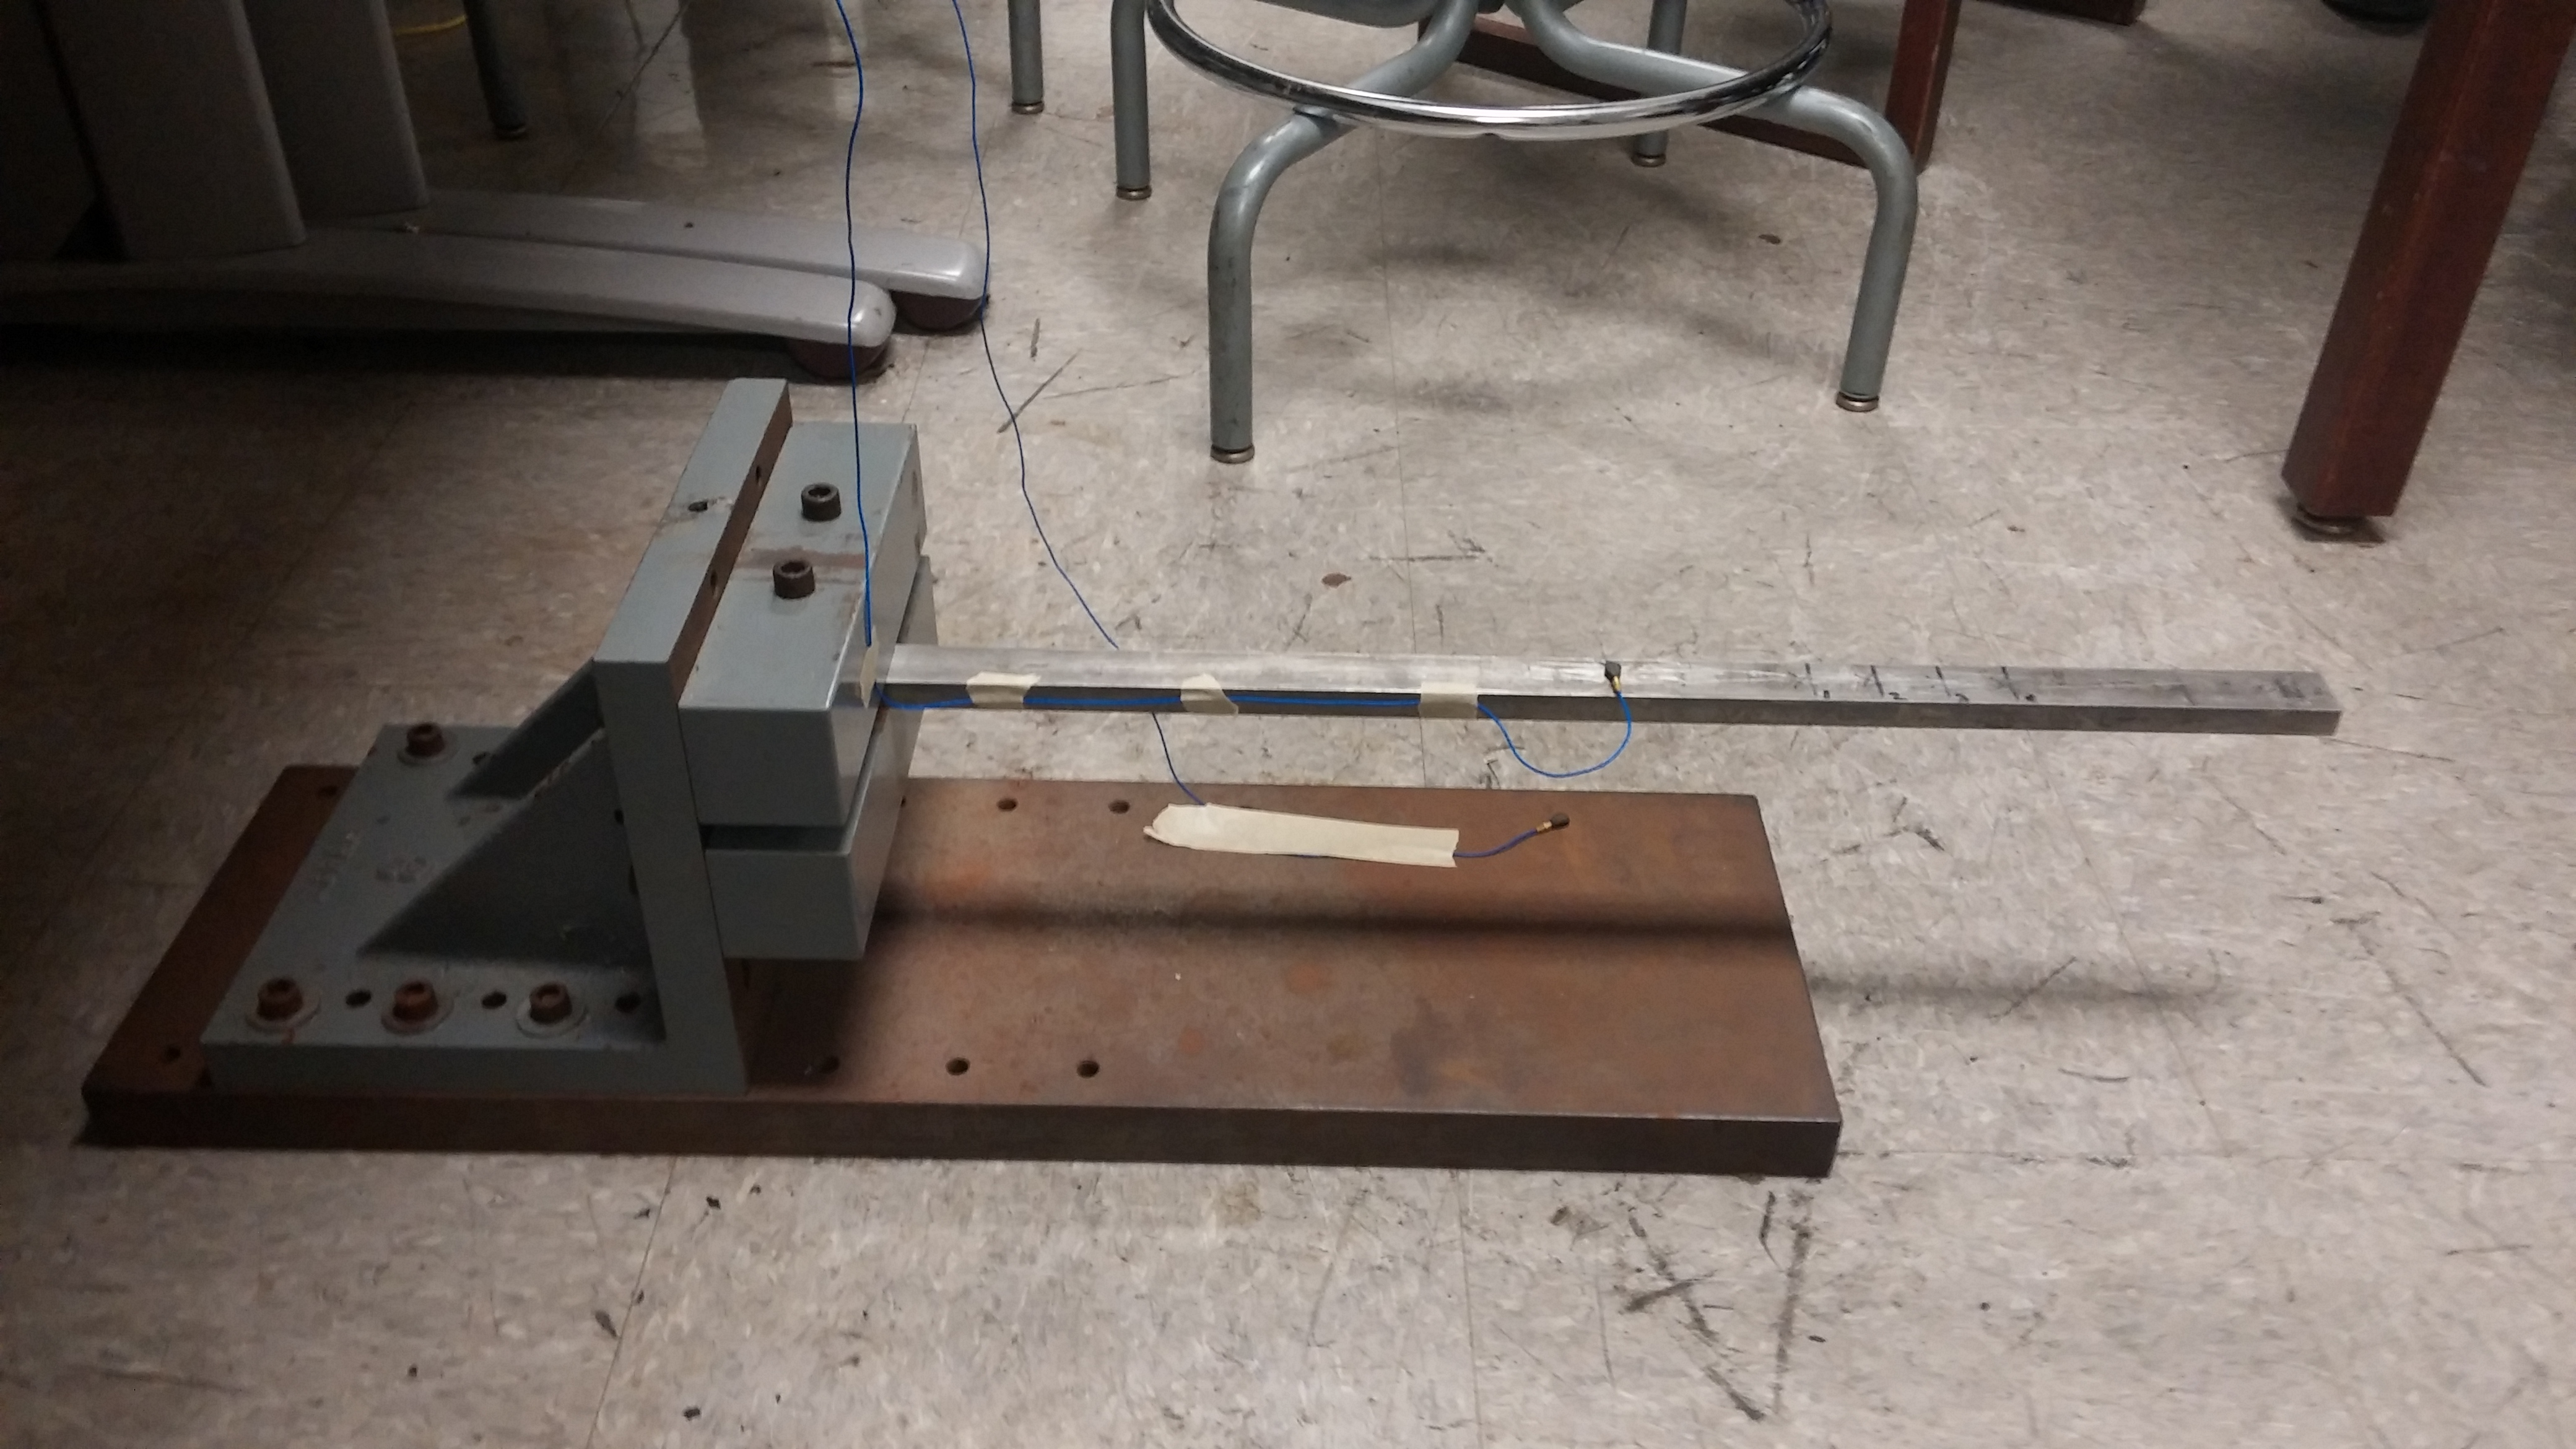
\includegraphics[height=4.0cm]{BeamSideProfile.jpg}
		\label{fig:beamSideProfile}
		}
		\caption{Cantilever Beam Setup}
	\end{figure}
%
The Figure shows a beam that is clamped to a fixture. In order to have proper cantilever beam response, the fixture must be very stiff. Applying this concept to Finite Element Analysis (FEA), the clamped end of the beam is simulated by applying a fixed constraint. This implies infinite stiffness at the boundary, which is never true in the real world but will agree well with the experimental results if the fixture is indeed stiff and has limited movement. Of course there are experimental cases where the boundary is not assumed to be rigid and it is important to capture this behavior in FEA with proper boundary treatments. In general, the goal is for the FEA to match the experimental set-up and not the other way around.
%
The following sections will discuss two experiments. The first experiments ensures that the fixture is made rigid and has very little motion. The second experimental set-up deliberately makes the fixture unstable by ensuring the ground contact is not stable and even. This in turn will allow for significant motion in the fixture itself during testing. Results from the two experiments will be discussed and compared to each other to determine the impact of poor base fixivity. Additionally, experimental results will be compared to analytical predictions.
%
%
\section*{Experimental Setup}
Experimental set-up for the two cases can be seen in Figure ~\ref{fig:test}. In Figure ~\ref{fig:BeamWtWeight2} the fixture is restrained by adding 50 pound weight on each corner of the base. Conversely, the set-up in Figure ~\ref{fig:BeamNoWeight} has the weight removed. In addition to this the base was placed on the section of the floor that is very uneven, which further destabilized the base. From this point on the two experiments will be refereed to as fixed and loose for clarity. It is also worth noting that the sensor cables were taped down to minimize noise due to cable movement.
%
	\begin{figure}[H]
		\centering
		\subfigure[Fixed cantilevered beam setup]
		{
		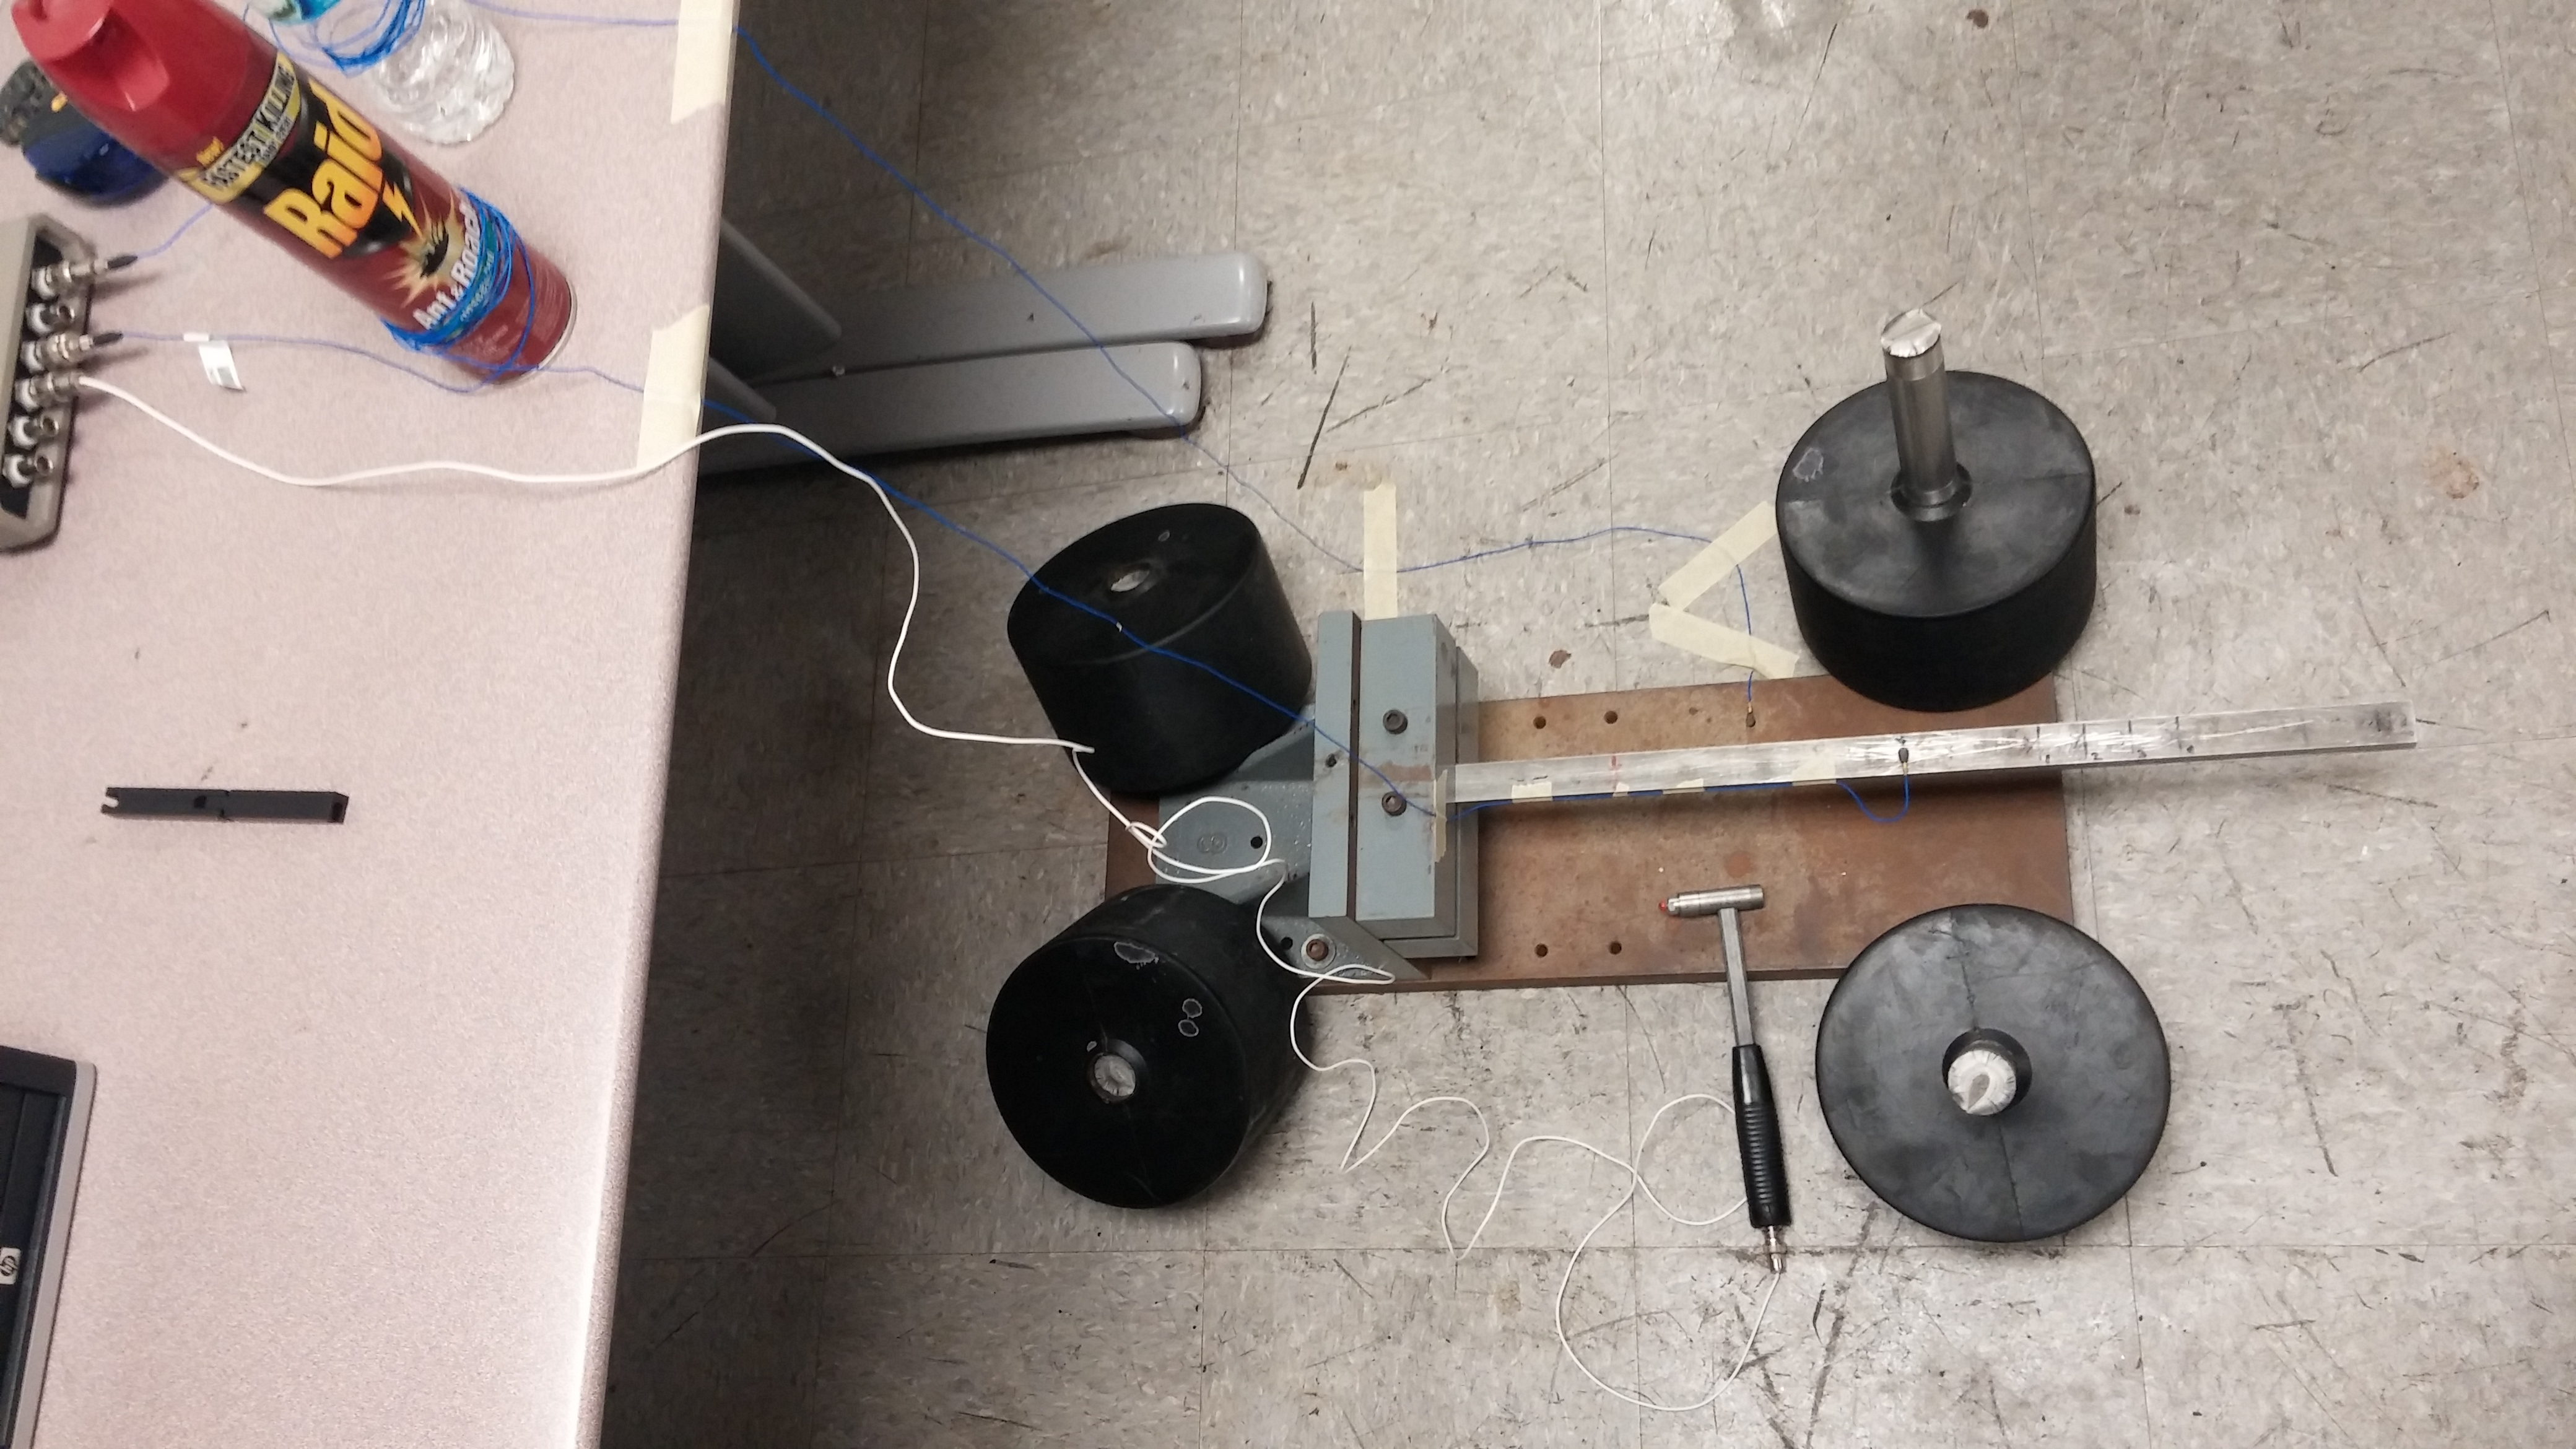
\includegraphics[height=5.50cm]{BeamWtWeight2.jpg}
		\label{fig:BeamWtWeight2}
		}
		\quad
		\subfigure[Loose cantilevered beam setup]
		{
		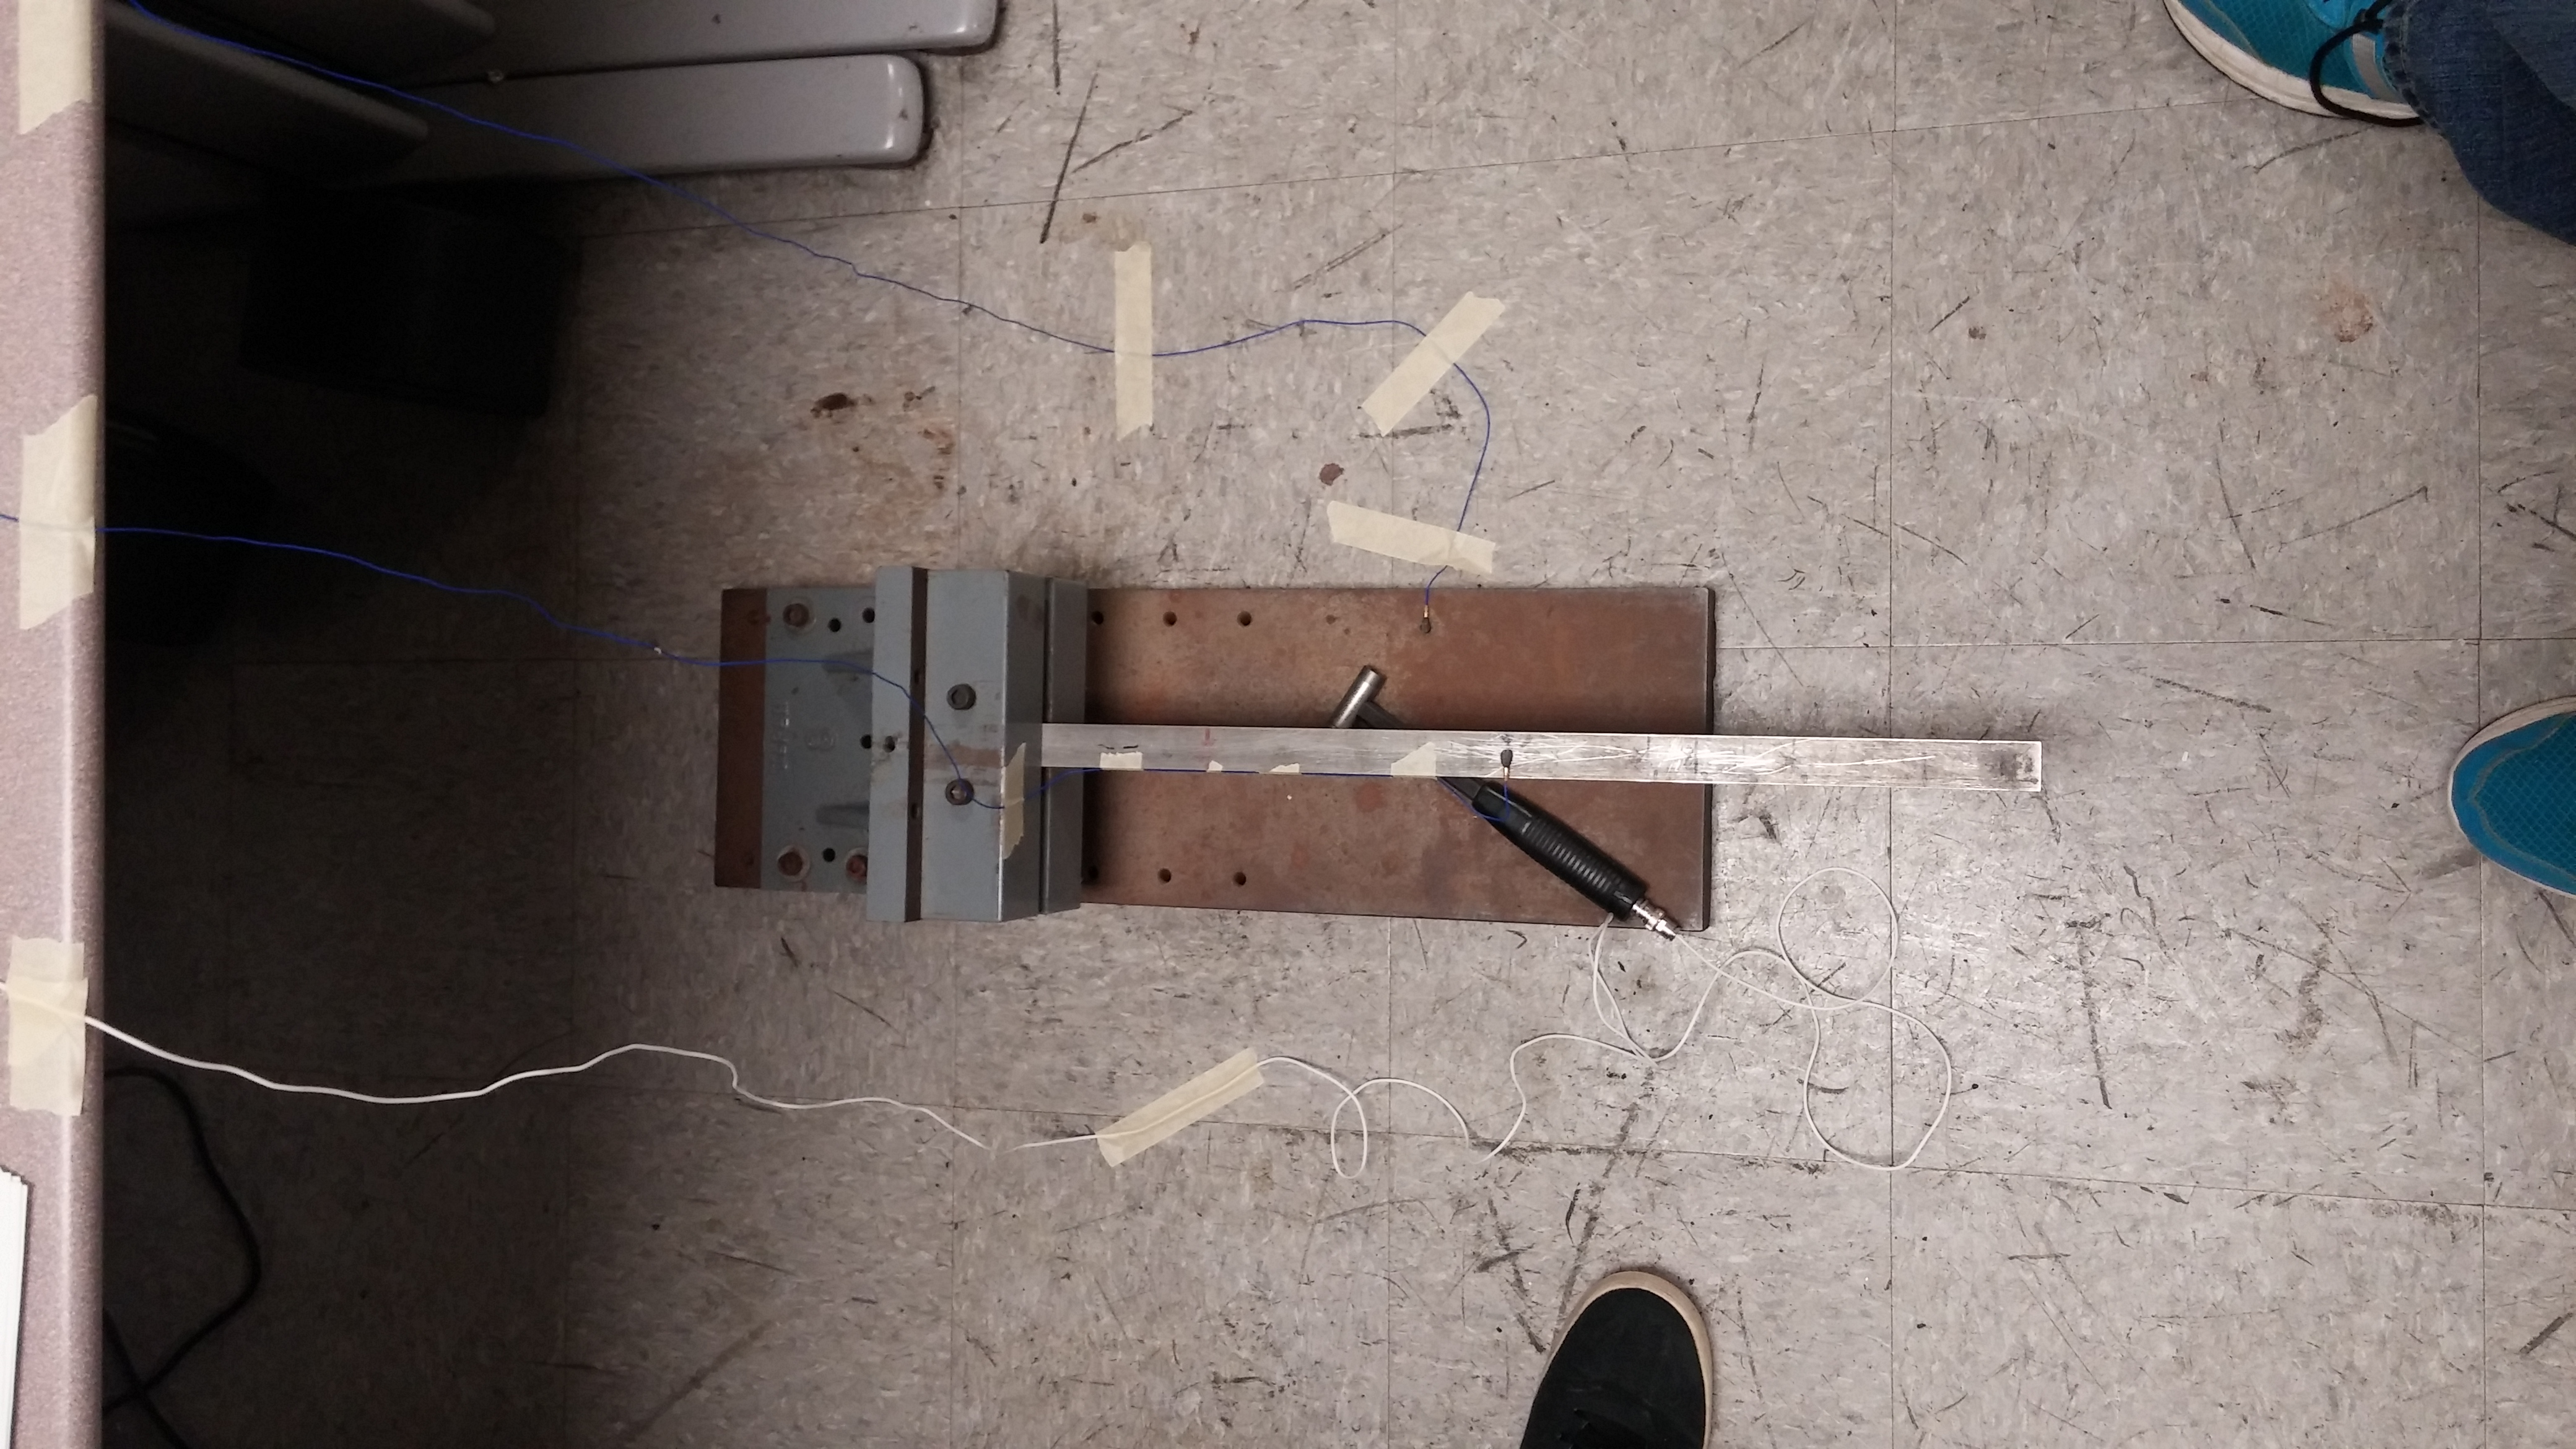
\includegraphics[height=5.50cm]{BeamNoWeight.jpg}
		\label{fig:BeamNoWeight}
		}
		\caption{Experimental setup for two cases}
		\label{fig:test}
	\end{figure}
%
Three signals were recorded during each experiment (1 input and 2 output). Signal definitions can be seen in the Table ~\ref{table:channelAssignments} below.
%
\begin{table}[H]
\centering
\begin{tabular}{ l | l }
	\hline                       
		Channel 1 & Hammer \\
	\hline
		Channel 2 & Beam Accelerometer \\
	\hline
		Channel 4 & Base Accelerometer \\
	\hline  
\end{tabular}
\caption{Channel Assignments}
\label{table:channelAssignments}
\end{table}
%
Channel assignments and sensor locations remained the same for both experiments in order to minimize errors due to set-up variation. For each case (fixed, loose) a total of 10 data sets were obtained. Five samples were obtained using hammer excitation at the base of the beam. The remaining five samples were obtained exciting the beam at location 4. Sensing and excitation locations are illustrated in Figure ~\ref{fig:topShot_mod} below.
%
	\begin{figure}[H]
		\centering
		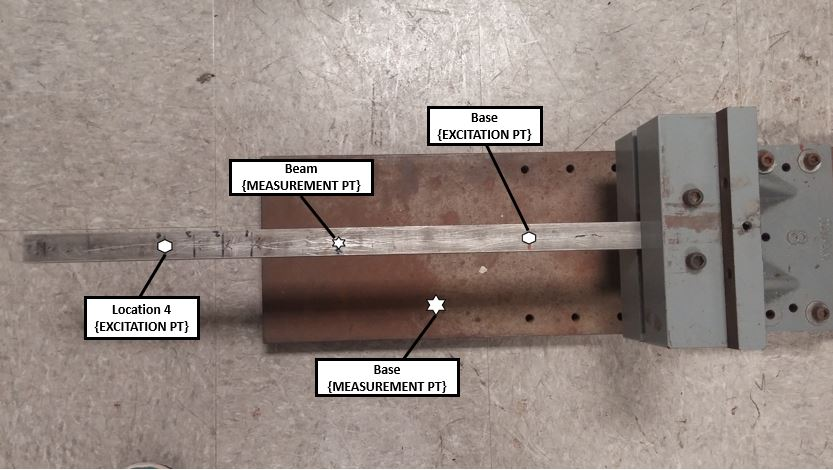
\includegraphics[height=5.0cm]{TopShot_mod.jpg}
		\label{fig:topShot_mod}
		\caption{Cantilever beam setup}
	\end{figure}
%
Time duration for each sample is 3.2 seconds. It was discovered at later time that the beam sensor was mounted upside down, which inverted the acceleration response. This, however, does not render the data useless. It is possible to invert the time history manually during the post-process stage. Another acceptable practice is to simply swap the operational order of input and output time histories when calculating cross spectrum densities (CSD) and frequency response functions (FRF).
\\
\\
In addition to the input and output data collected, two data series were obtained for the hammer and sensors while they were resting in their respective boxes. Intention for this data is to modify the response signals during the post process phase in an attempt to reduce noise before calculating CSD's and FRF's.
%
%
\section*{Data Inspection}
Input and output time histories were plotted to confirm proper response characteristics. In general the response behaved in an expected manner when compared to other cantilever beam data. For both base and LOC4 beam responses there was a vertical shift in the data, which prevented symmetric oscillation about the x-axis. This shift was observed in the response data of the sensors while they were sitting in their boxes. For this case decision was made to use this data in order to shift the beam responses closer to the x-axis. Results of this operation can be seen in the Figure ~\ref{fig:weightTimeResponse} below for the fixed base condition.
%
	\begin{figure}[H]
		\centering
		\subfigure[Base excitation response for the weighted fixture]
		{
		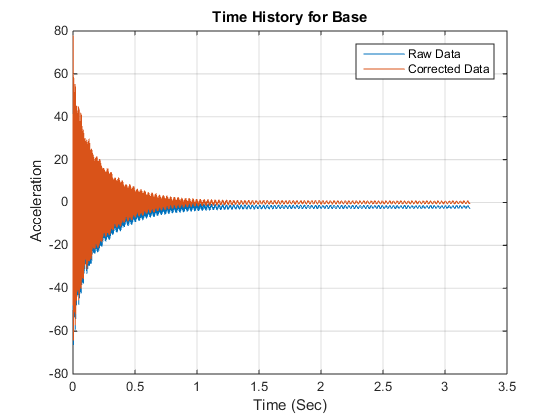
\includegraphics[height=5.50cm]{base_wt_weight_timeData.jpg}
		\label{fig:baseTimeData}
		}
		\quad
		\subfigure[LOC4 excitation response for the weighted fixture]
		{
		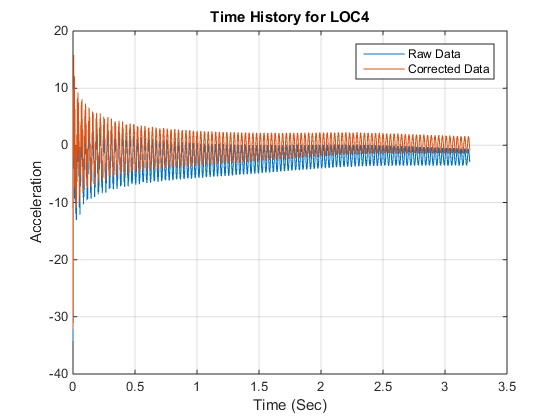
\includegraphics[height=5.50cm]{LOC4_wt_weight_timeData.jpg}
		\label{fig:LOC4TimeData}
		}
		\caption{Raw and shiffted response histories for the cantilever beam (FIXED)}
		\label{fig:weightTimeResponse}
	\end{figure}
%
In Figure ~\ref{fig:LOC4TimeData} it becomes evident that the sensor mounted on the beam is indeed inverted since the highest amplitude occurs in the negative half of the plot. It is also evident that the modified data now looks more symmetric about the x-axis. In similar manner the input time response also posses the vertical shift, which was removed from the data using the raw input signal from the hammer while it was sitting in its respective box. The results for the shifted input signal can be seen in Figure ~\ref{fig:weightInputResponse}.
%
	\begin{figure}[H]
		\centering
		\subfigure[Input signal for base excitation]
		{
		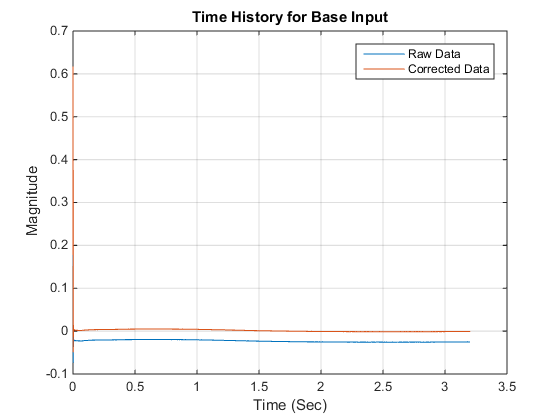
\includegraphics[height=5.50cm]{base_wt_weight_input.jpg}
		\label{fig:baseInputData}
		}
		\quad
		\subfigure[Input signal for LOC4 excitation]
		{
		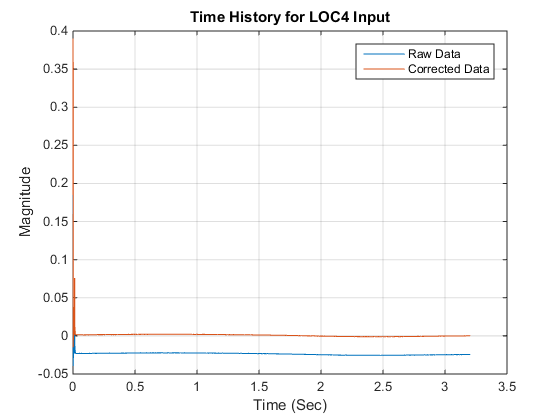
\includegraphics[height=5.50cm]{LOC4_wt_weight_input.jpg}
		\label{fig:LOC4InputData}
		}
		\caption{Raw and shifted input signals (FIXED)}
		\label{fig:weightInputResponse}
	\end{figure}
%
The hammer strike appears well defined for both the base and LOC4 excitation. There is however a small double strike that consistently occurred while exciting LOC4.
\\
\\
In the next subsection similar plots are presented for the loose condition. One thing that is quite apparent is the fact the system damping is significantly higher due to the fact the response dies off in about 1.0-1.5 seconds. This is mainly due to pronounced fixture movement, which acts to remove energy from the system. This effect along with vertical shift of the data can be seen in Figure ~\ref{fig:looseTimeResponse} below.
%
	\begin{figure}[H]
		\centering
		\subfigure[Base excitation response for the loose fixture]
		{
		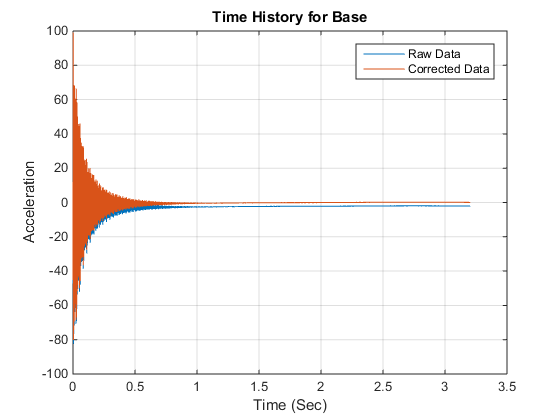
\includegraphics[height=5.50cm]{base_wo_weight_timeData.jpg}
		\label{fig:baseTimeData2}
		}
		\quad
		\subfigure[LOC4 excitation response for the loose fixture]
		{
		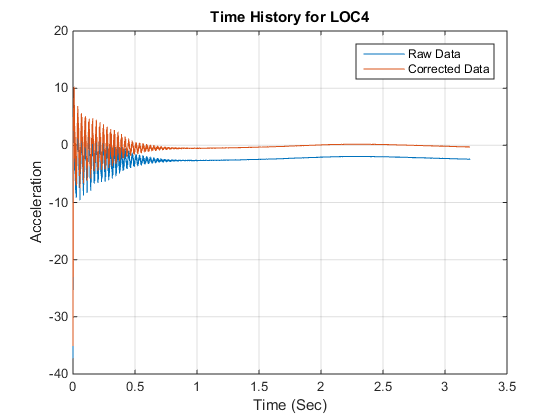
\includegraphics[height=5.50cm]{LOC4_wo_weight_timeData.jpg}
		\label{fig:LOC4TimeData2}
		}
		\caption{Raw and shifted response histories for the cantilever beam (LOOSE)}
		\label{fig:looseTimeResponse}
	\end{figure}
%
The input signals did not exhibit any notable differences when compared to the fixed base condition. Input signal for LOC4 shows a double strike feature, which was also noted for the input signal of the fixed base experiments. Input signals for the loose condition were also shifted and those results can be seen in Figure ~\ref{fig:looseInputResponse2}.
%
	\begin{figure}[H]
		\centering
		\subfigure[Input signal for base excitation]
		{
		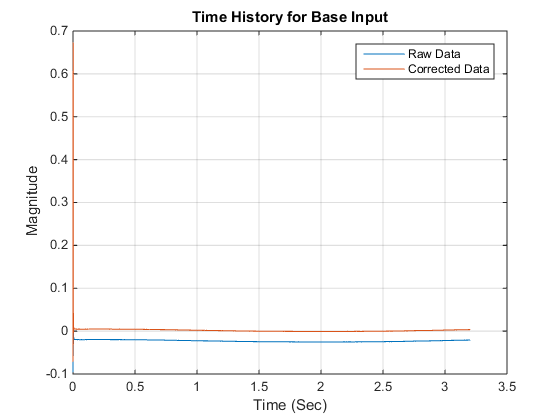
\includegraphics[height=5.50cm]{base_wo_weight_input.jpg}
		\label{fig:baseInputData2}
		}
		\quad
		\subfigure[Input signal for LOC4 excitation]
		{
		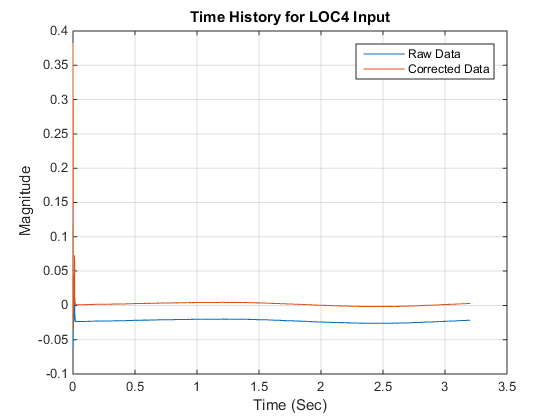
\includegraphics[height=5.50cm]{LOC4_wo_weight_input.jpg}
		\label{fig:LOC4InputData2}
		}
		\caption{Raw and shifted input signals (LOOSE)}
		\label{fig:looseInputResponse2}
	\end{figure}
%
In the next section both shifted and raw time data were used to generate FRF's for the FIXED and LOOSE fixture condition.
%
%
\section*{Data Analysis}
In this section vibration toolbox was used to calculate all the items listed in Table ~\ref{table:performedCalculations}. Both raw and shifted data were used for both experimental setups. In general, shifting the data did not change the calculations to any significant degree. The effect of the LOOSE fixture condition seems to be more pronounced when the beam is excited at LOC4. Each calculation performed in Matlab used 5 data samples.
%
\begin{table}[H]
\centering
\begin{tabular}{ l | l }
		\textbf{Calculation} & \textbf{Number of Samples} \\
	\hline                       
		Cross Spectrum Density (CSD) & 5 samples \\
	\hline
		Auto Spectrum Density (input) (ASD) & 5 samples \\
	\hline
		Auto Spectrum Density (output) (ASD) & 5 samples \\
	\hline  
		Frequency Response Function (H1, H2) & 5 samples \\
	\hline  
		Coherence & 5 samples \\
\end{tabular}
\caption{Performed calculations}
\label{table:performedCalculations}
\end{table}
%
For the sake of brevity only pertinent plots will be shown in this section. The remaining plots can be found in the Appendix. First set of plots shown pertain to the base excitation. Starting with the plots of the CSD, Figure ~\ref{fig:baseCSDFigs} shows the impact of two different fixture setting along with data correction effects.
%
	\begin{figure}[H]
		\centering
		\subfigure[CSD for base excitation using raw data (FIXED)]
		{
		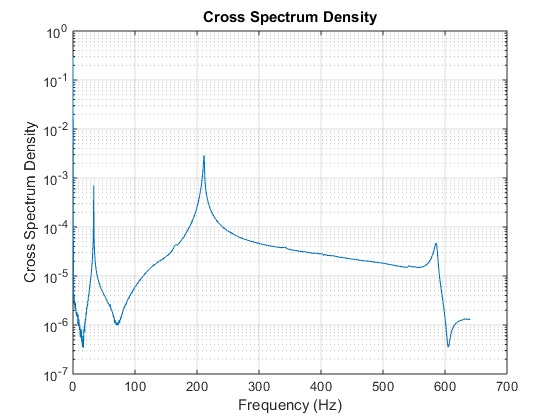
\includegraphics[height=5.50cm]{baseR_wtWeight_CSD.jpg}
		\label{fig:baseR_wtWeight_CSD}
		}
		\quad
		\subfigure[CSD for base excitation using raw data (LOOSE)]
		{
		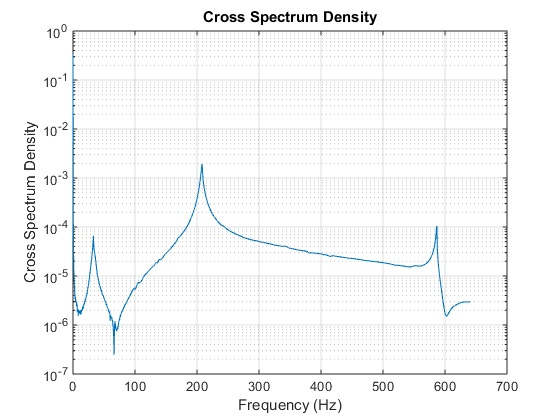
\includegraphics[height=5.50cm]{baseR_woWeight_CSD.jpg}
		\label{fig:baseR_woWeight_CSD}
		}
		\quad
		\subfigure[CSD for base excitation using corrected data (FIXED)]
		{
		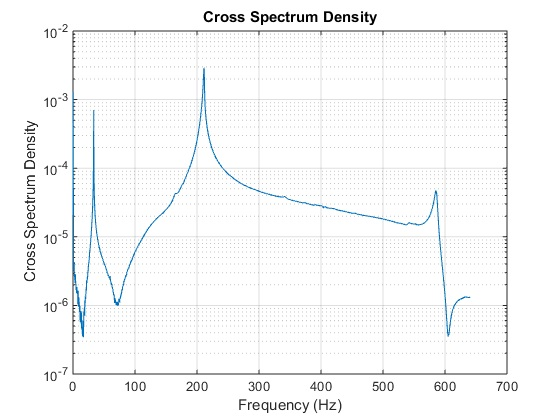
\includegraphics[height=5.50cm]{baseC_wtWeight_CSD.jpg}
		\label{fig:baseC_wtWeight_CSD}
		}
		\quad
		\subfigure[CSD for base excitation using corrected data(LOOSE)]
		{
		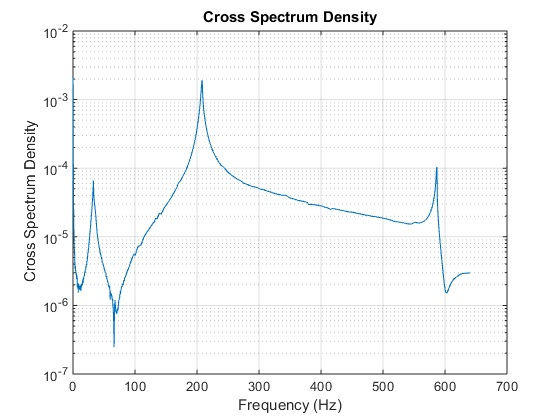
\includegraphics[height=5.50cm]{baseC_woWeight_CSD.jpg}
		\label{fig:baseC_woWeight_CSD}
		}
		\caption{CSD plots for base excitation. Results shown for FIXED and LOOSE 					condition.}
		\label{fig:baseCSDFigs}
	\end{figure}
%
Shifting the data had no appreciable impact on the CSD plots when comparing Figures ~\ref{fig:baseR_wtWeight_CSD}, ~\ref{fig:baseC_wtWeight_CSD} and ~\ref{fig:baseR_woWeight_CSD}, ~\ref{fig:baseC_woWeight_CSD}. On the other hand, fixture setting did show additional noise for the LOOSE condition. This noise is especially evident at the zero located near 75 Hz. Even with the additional noise the poles are well defined for all cases. There appears to be no shift in the natural frequency locations.
\\
\\
Figure ~\ref{fig:baseH1H2Figs} shows the H1 and H2 FRF estimations along with the phase plots.
%
	\begin{figure}[H]
		\centering
		\subfigure[H1 and H2 for base excitation using raw data (FIXED)]
		{
		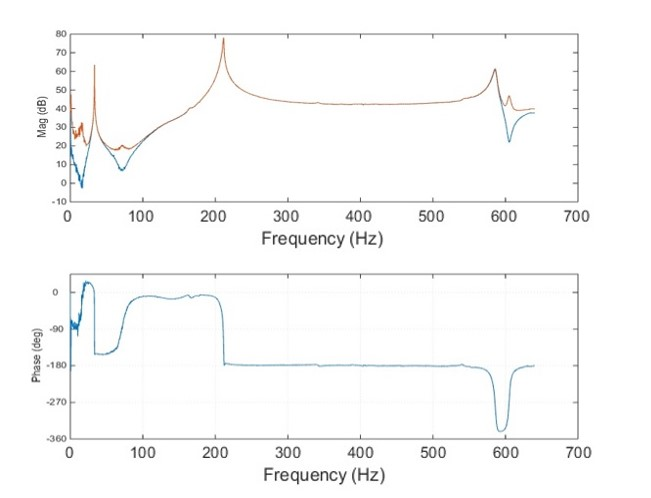
\includegraphics[height=4.60cm]{baseR_wtWeight_H1_H2_2.jpg}
		\label{fig:baseR_wtWeight_H1_H2_2}
		}
		\quad
		\subfigure[H1 and H2 for base excitation using raw data (LOOSE)]
		{
		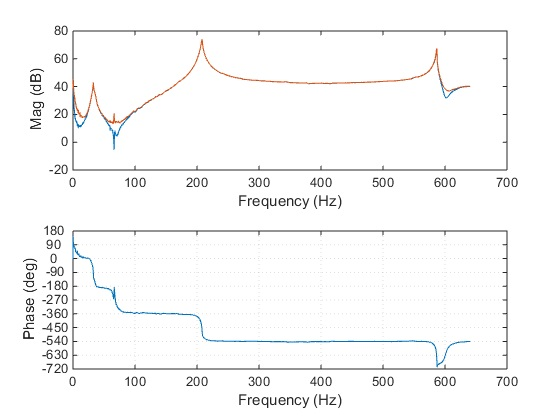
\includegraphics[height=4.60cm]{baseR_woWeight_H1_H2.jpg}
		\label{fig:baseR_woWeight_H1_H2}
		}
		\quad
		\subfigure[H1 and H2 for base excitation using corrected data (FIXED)]
		{
		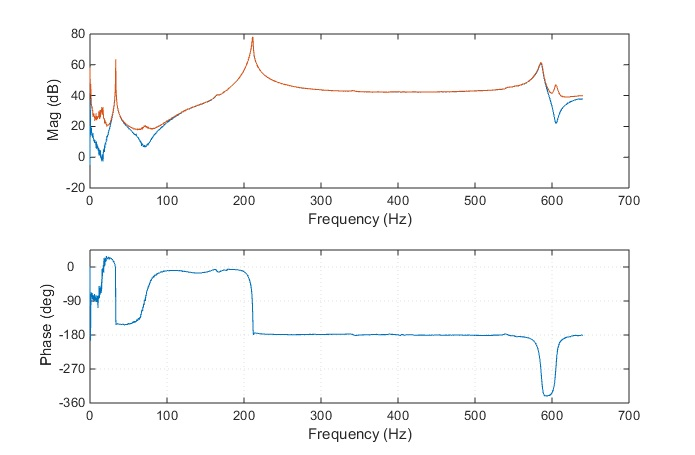
\includegraphics[height=4.50cm]{baseC_wtWeight_H1_H2.jpg}
		\label{fig:baseC_wtWeight_H1_H2}
		}
		\quad
		\subfigure[H1 and H2 for base excitation using corrected data(LOOSE)]
		{
		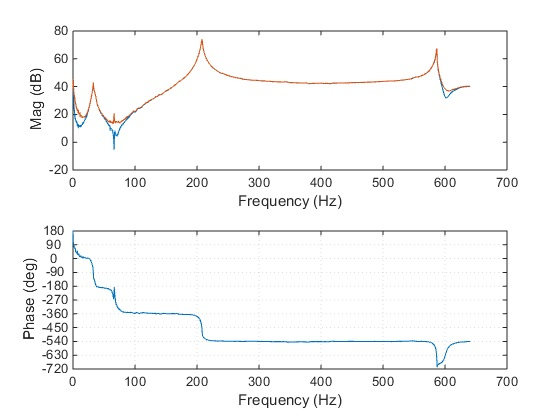
\includegraphics[height=4.50cm]{baseC_woWeight_H1_H2.jpg}
		\label{fig:baseC_woWeight_H1_H2}
		}
		\caption{H1 and H2 plots for base excitation. Results shown for FIXED and LOOSE 					condition.}
		\label{fig:baseH1H2Figs}
	\end{figure}
%
As was the case for the CSD plots in Figure~\ref{fig:baseCSDFigs} there is additional noise present near the zero located at 75 Hz. The additional noise impact can be clearly seen when looking at the phase plots of Figures ~\ref{fig:baseR_wtWeight_H1_H2_2}, ~\ref{fig:baseR_woWeight_H1_H2}, ~\ref{fig:baseC_wtWeight_H1_H2},  ~\ref{fig:baseC_woWeight_H1_H2}. For the FIXED case there is a positive phase shift at the 75 Hz zero location. Conversely, for the LOOSE case the additional noise causes the calculation to think there is an additional pole at 75 Hz. As a result, the phase diagram shows a negative phase shift at 75 Hz. At the zero location system displacement is very low and can be susceptible to noise errors. For the LOOSE case it is possible that the instability of the fixture caused the error floor to be in the same amplitude range as the actual zero measurement from the beam. This could lead to the discrepancy witnessed in the phase diagrams.
\\
\\
Finally the coherence plots are shown in Figure below.
%
	\begin{figure}[H]
		\centering
		\subfigure[Coherence for base excitation using raw data (FIXED)]
		{
		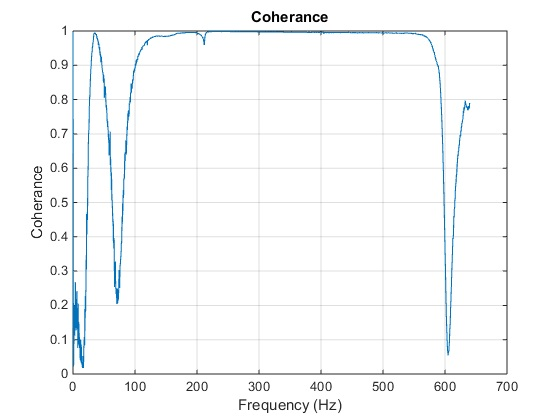
\includegraphics[height=5.50cm]{baseR_wtWeight_coherance.jpg}
		\label{fig:baseR_wtWeight_coherance}
		}
		\quad
		\subfigure[Coherence for base excitation using raw data (LOOSE)]
		{
		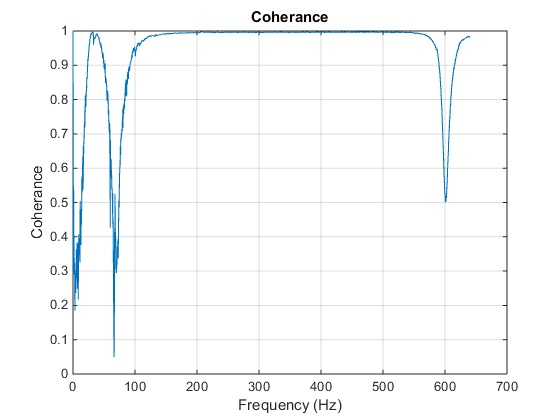
\includegraphics[height=5.50cm]{baseR_woWeight_coherance.jpg}
		\label{fig:baseR_woWeight_coherance}
		}
%		\caption{}
		\label{fig:baseCohFigs1}
	\end{figure}
	\begin{figure}[H]
		\centering
		\subfigure[Coherence for base excitation using corrected data (FIXED)]
		{
		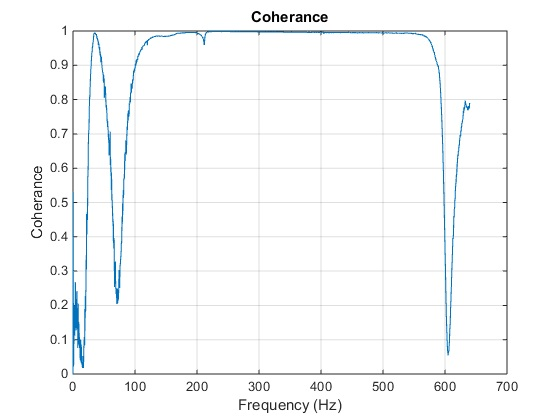
\includegraphics[height=5.50cm]{baseC_wtWeight_coherance.jpg}
		\label{fig:baseC_wtWeight_coherance}
		}
		\quad
		\subfigure[Coherence for base excitation using corrected data(LOOSE)]
		{
		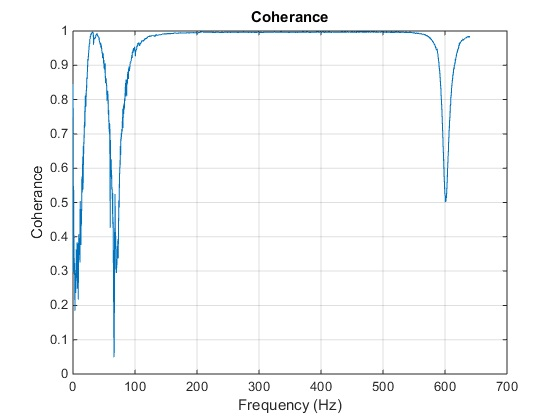
\includegraphics[height=5.50cm]{baseC_woWeight_coherance.jpg}
		\label{fig:baseC_woWeight_coherance}
		}
		\caption{Coherence plots for base excitation. Results shown for FIXED and LOOSE 					condition.}
		\label{fig:baseCohFigs2}
	\end{figure}
%
Coherence plots for all cases look similar with respect to each other. Very good coherence is obtained from 100-500 Hz. Remaining frequency range is not considered in the analysis as it is the last 20$\%$ of the frequency bandwidth.
%
\\
\\
In the following subsection same plots are provided for the beam response when excited at LOC4. Figure~\ref{fig:LOC4CSDFigs} below shows plots for the CSD's.
%
	\begin{figure}[H]
		\centering
		\subfigure[CSD for base excitation using raw data (FIXED)]
		{
		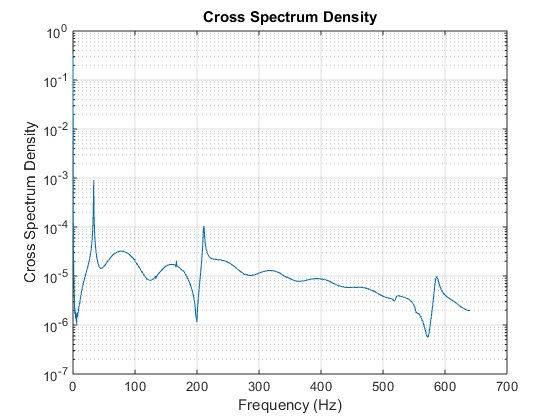
\includegraphics[height=5.50cm]{LOC4R_wtWeight_CSD.jpg}
		\label{fig:LOC4R_wtWeight_CSD}
		}
		\quad
		\subfigure[CSD for base excitation using raw data (LOOSE)]
		{
		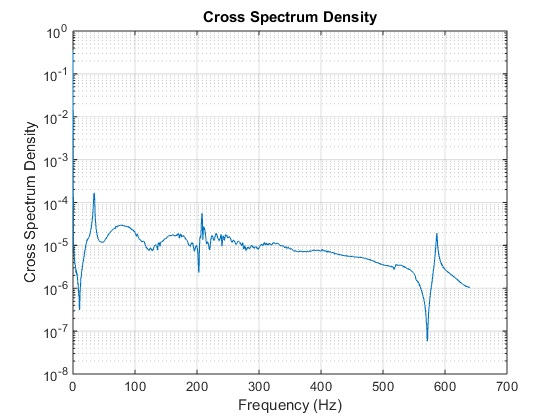
\includegraphics[height=5.50cm]{LOC4R_woWeight_CSD.jpg}
		\label{fig:LOC4R_woWeight_CSD}
		}
		\quad
		\subfigure[CSD for base excitation using corrected data (FIXED)]
		{
		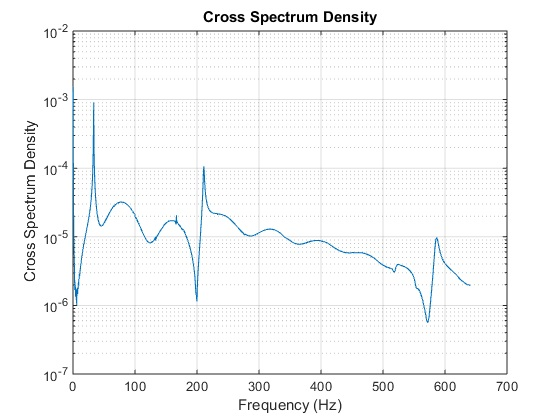
\includegraphics[height=5.50cm]{LOC4C_wtWeight_CSD.jpg}
		\label{fig:LOC4C_wtWeight_CSD}
		}
		\quad
		\subfigure[CSD for base excitation using corrected data(LOOSE)]
		{
		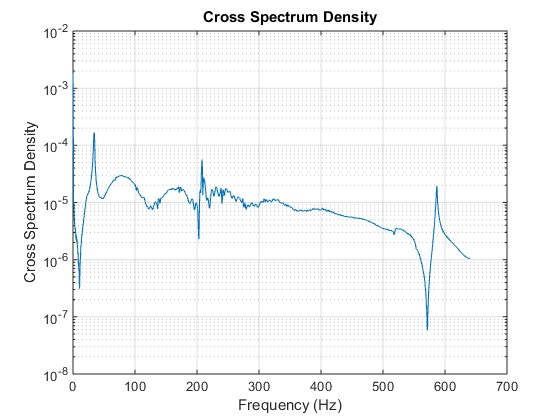
\includegraphics[height=5.50cm]{LOC4C_woWeight_CSD.jpg}
		\label{fig:LOC4C_woWeight_CSD}
		}
		\caption{CSD plots for base excitation. Results shown for FIXED and LOOSE 					condition.}
		\label{fig:LOC4CSDFigs}
	\end{figure}
%
At the 200 Hz location there is almost a pole/zero cancellation. All the plots show this property but the LOOSE plots have significant amount of noise in this region. If no FIXED data was available for comparison this aspect of the system response can be easily missed. Comparing Figure~\ref{fig:LOC4CSDFigs} to Figure~\ref{fig:baseCSDFigs} there is noticeable waviness in Figure~\ref{fig:LOC4CSDFigs}. This can be attributed to the over-damped type response for the LOOSE time data. Since the response dies off relatively fast (in about 1 second) there is not enough time data to get sufficient frequency resolution. In turn there appears to be leakage to surrounding frequency values.
\\
\\
Next set of plots show the H1 and H2 FRF estimates for LOC4 excitation.
%
	\begin{figure}[H]
		\centering
		\subfigure[H1 and H2 for LOC4 excitation using raw data (FIXED)]
		{
		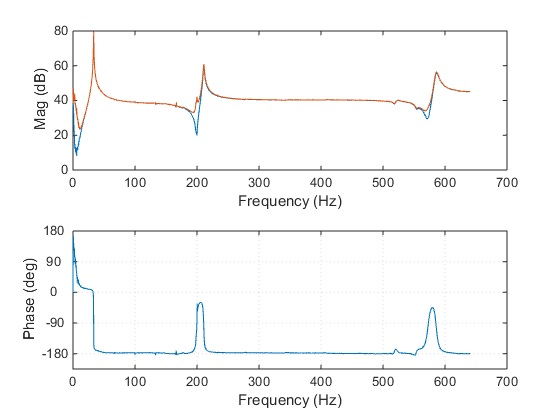
\includegraphics[height=5.50cm]{LOC4R_wtWeight_H1_H2.jpg}
		\label{fig:LOC4R_wtWeight_H1_H2}
		}
		\quad
		\subfigure[H1 and H2 for LOC4 excitation using raw data (LOOSE)]
		{
		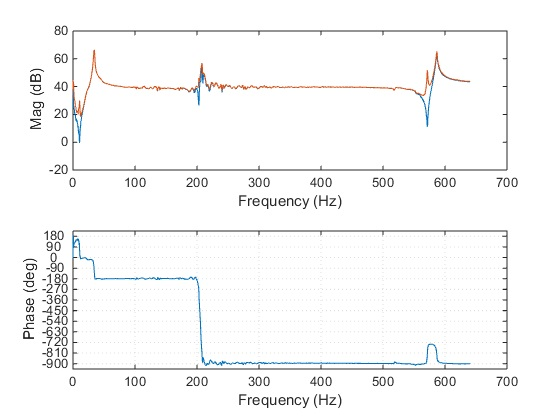
\includegraphics[height=5.50cm]{LOC4R_woWeight_H1_H2.jpg}
		\label{fig:LOC4R_woWeight_H1_H2}
		}
		\quad
		\subfigure[H1 and H2 for LOC4 excitation using corrected data (FIXED)]
		{
		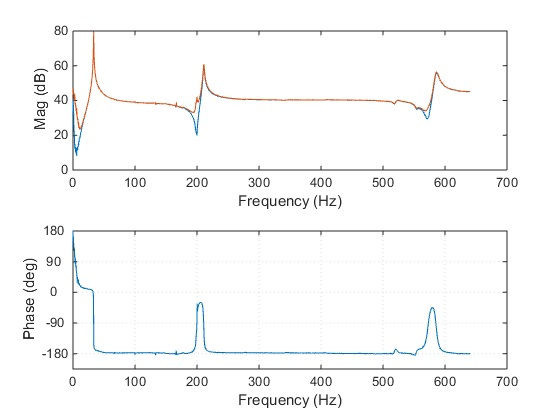
\includegraphics[height=5.50cm]{LOC4C_wtWeight_H1_H2.jpg}
		\label{fig:LOC4C_wtWeight_H1_H2}
		}
		\quad
		\subfigure[H1 and H2 for LOC4 excitation using corrected data(LOOSE)]
		{
		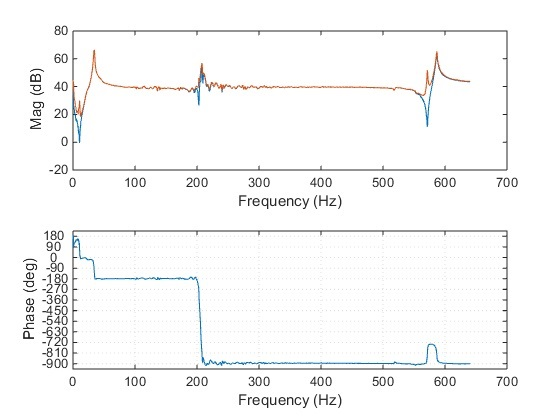
\includegraphics[height=5.50cm]{LOC4C_woWeight_H1_H2.jpg}
		\label{fig:LOC4C_woWeight_H1_H2}
		}
		\caption{H1 and H2 plots for LOC4 excitation. Results shown for FIXED and LOOSE condition.}
		\label{fig:LOC4H1H2Figs}
	\end{figure}
%
The phase diagram of Figures~\ref{fig:LOC4R_wtWeight_H1_H2} and ~\ref{fig:LOC4C_wtWeight_H1_H2} shows how close the FRF was to having a pole/zero cancelation. Additionally, when looking at the FRF and phase plots of the LOOSE response (~\ref{fig:LOC4R_woWeight_H1_H2}, ~\ref{fig:LOC4C_woWeight_H1_H2}) the zero is completly masked by the noise. Furthermore, it appears from the plots that there are two closely spaced poles, which should not be the case.
%
\\
\\
Finally the coherence plots for the LOC4 excitation are shown in Figure~\ref{fig:LOC4CohFigs2}.
%
	\begin{figure}[H]
		\centering
		\subfigure[Coherence for LOC4 excitation using raw data (FIXED)]
		{
		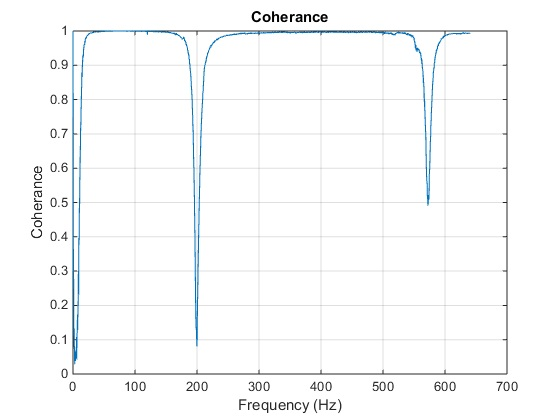
\includegraphics[height=5.50cm]{LOC4R_wtWeight_coherance.jpg}
		\label{fig:LOC4R_wtWeight_coherance}
		}
		\quad
		\subfigure[Coherence for LOC4 excitation using raw data (LOOSE)]
		{
		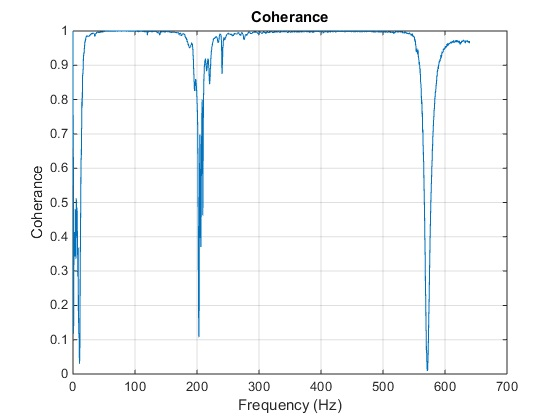
\includegraphics[height=5.50cm]{LOC4R_woWeight_coherance.jpg}
		\label{fig:LOC4R_woWeight_coherance}
		}
%		\caption{}
%		\label{fig:baseCohFigs1}
%	\end{figure}
%	\begin{figure}[H]
%		\centering
		\subfigure[Coherence for LOC4 excitation using corrected data (FIXED)]
		{
		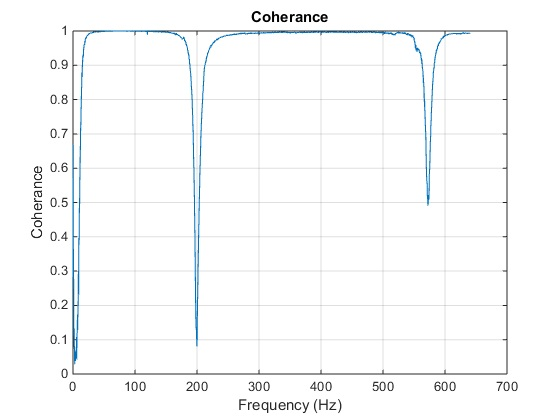
\includegraphics[height=5.50cm]{LOC4C_wtWeight_coherance.jpg}
		\label{fig:LOC4C_wtWeight_coherance}
		}
		\quad
		\subfigure[Coherence for LOC4 excitation using corrected data(LOOSE)]
		{
		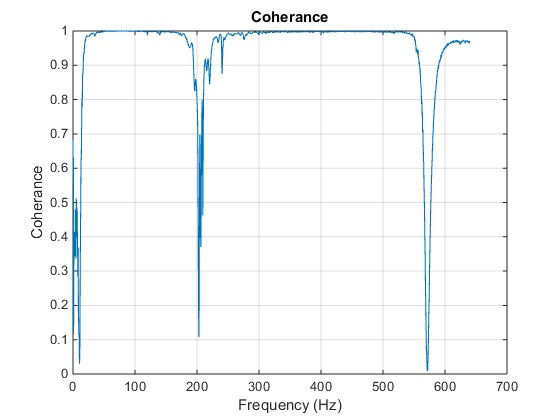
\includegraphics[height=5.50cm]{LOC4C_woWeight_coherance.jpg}
		\label{fig:LOC4C_woWeight_coherance}
		}
		\caption{Coherence plots for LOC4 excitation. Results shown for FIXED and LOOSE condition.}
		\label{fig:LOC4CohFigs2}
	\end{figure}
%
The coherence plots show excellent behavior across the entire frequency range. Drops observed at the pole locations are to be expected. Plots in Figures~\ref{fig:LOC4R_woWeight_coherance} and~\ref{fig:LOC4C_woWeight_coherance} have noisy behavior, which is due to the LOOSE condition of the fixture.
%
%
\section*{Summary}
%
Experiments were conducted using two distinct fixture set-ups. For the first experimental set-up the fixture was well grounded and additionally supported by adding 50 pound weights on each corner. This condition was dubbed as "FIXED". For the second set-up the weights were not used. Additionally, the fixture for the second case was purposefully placed on the uneven area of the floor, which further exacerbated fixture instability. This case was dubbed as "LOOSE".  
\\
\\
For both cases, sensors and excitation locations remained the same and are depicted in Figure~\ref{fig:topShot_mod}. For each of the four combinations 5 experiments were conducted. This resulted in a total of 20 data sets for analysis. The goal of the study is to ascertain the impact of poor fixture stability on the beam response. In addition, a secondary goal was to determine the significance shifting data to account for the drift in the input and sensor signals.  
\\
\\
Experimental data was post-processed and their respective responses plotted with the help of the vibration toolbox. Both raw and corrected data sets were evaluated. Correcting the data for the sensor drift had no significant impact on the structure of the CSD, FRF, and coherence plots. Therefore, for this case the exercise was superfluous. 
\\
\\
Influence of fixture stability did have a profound impact on the beam response and its respective FRF estimations. For base and LOC4 data sets the zero definitions were 'smeared' by the additional noise generated by the unstable fixture. Phase diagrams for all LOOSE calculations failed to identify the zero locations. Moreover, it also seems to add an artificial pole at the zero location. For LOC4 FRF estimates there was a near pole/zero calculation, which is evident in the phase diagrams of the FIXED data sets. The coherence plots were of very good quality even for the LOOSE data sets. However, they did appear more noisy near the pole locations. In conclusion ensuring good fixture grounding is quite essential to obtaining accurate system response of the cantilever beam. If FIXED data was not available for comparison it would have been very easy to miss the zero of the system. Additionally, LOOSE data seems to have an artificial pole in the zero region. Surprisingly the natural frequency peaks did not have any significant shift between FIXED and LOOSE data.
\\
\\
Appendix contains the auto spectrum density plots for all cases to serve as reference.
%
%----------------------------------------------------------------------------------------
%	References #
%----------------------------------------------------------------------------------------
%\bibliographystyle{aiaa}  
%\bibliography{ref}
%----------------------------------------------------------------------------------------
%	PROBLEM #
%----------------------------------------------------------------------------------------
\section*{Appendix}
%
	\begin{figure}[H]
		\centering
		\subfigure[Input ASD for base excitation using raw data (FIXED)]
		{
		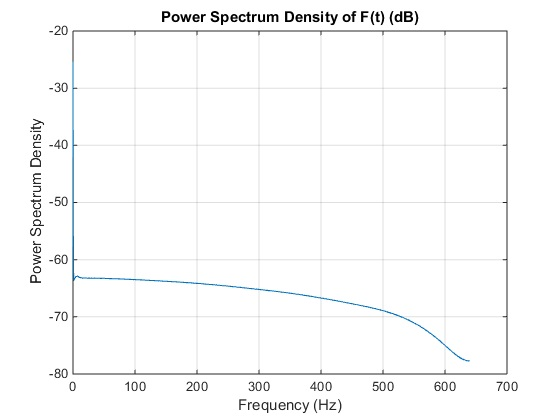
\includegraphics[height=5.50cm]{baseR_wtWeight_ASDinput.jpg}
		\label{fig:baseR_wtWeight_ASDinput}
		}
		\quad
		\subfigure[Input ASD for base excitation using raw data (LOOSE)]
		{
		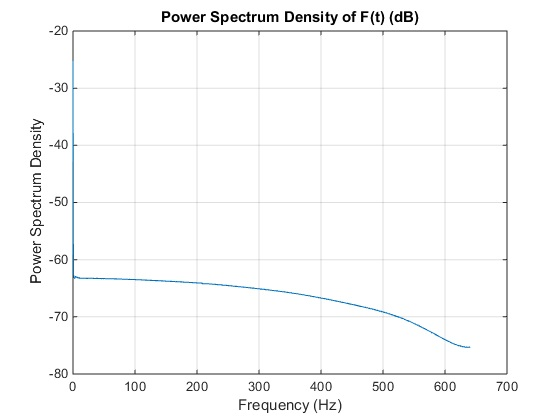
\includegraphics[height=5.50cm]{baseR_woWeight_ASDinput.jpg}
		\label{fig:baseR_woWeight_ASDinput}
		}
		\quad
		\subfigure[Input ASD for base excitation using corrected data (FIXED)]
		{
		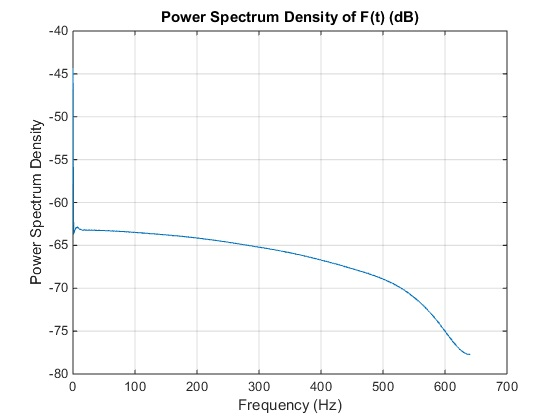
\includegraphics[height=5.50cm]{baseC_wtWeight_ASDinput.jpg}
		\label{fig:baseC_wtWeight_ASDinput}
		}
		\quad
		\subfigure[Input ASD for base excitation using corrected data(LOOSE)]
		{
		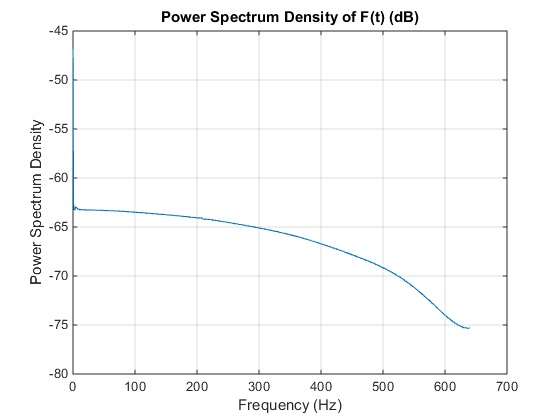
\includegraphics[height=5.50cm]{baseC_woWeight_ASDinput.jpg}
		\label{fig:baseC_woWeight_ASDinput}
		}
		\caption{Input ASD plots for base excitation. Results shown for FIXED and LOOSE condition.}
		\label{fig:InputASDBaseFigs}
	\end{figure}
%
	\begin{figure}[H]
		\centering
		\subfigure[Output ASD for base excitation using raw data (FIXED)]
		{
		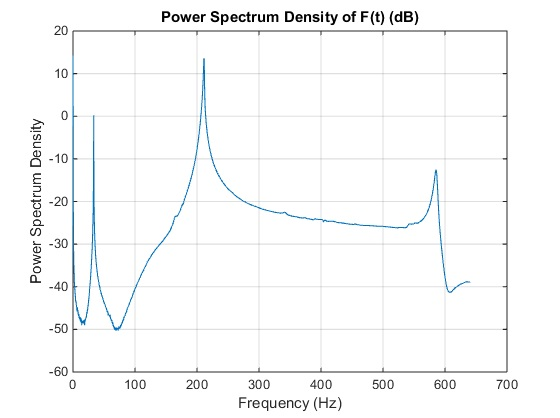
\includegraphics[height=5.50cm]{baseR_wtWeight_ASDoutput.jpg}
		\label{fig:baseR_wtWeight_ASDoutput}
		}
		\quad
		\subfigure[Output ASD for base excitation using raw data (LOOSE)]
		{
		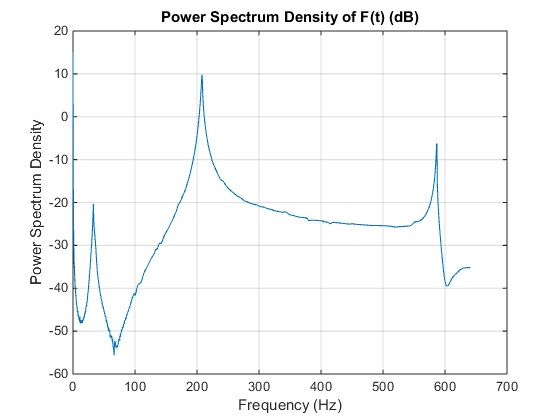
\includegraphics[height=5.50cm]{baseR_woWeight_ASDoutput.jpg}
		\label{fig:baseR_woWeight_ASDoutput}
		}
		\quad
		\subfigure[Output ASD for base excitation using corrected data (FIXED)]
		{
		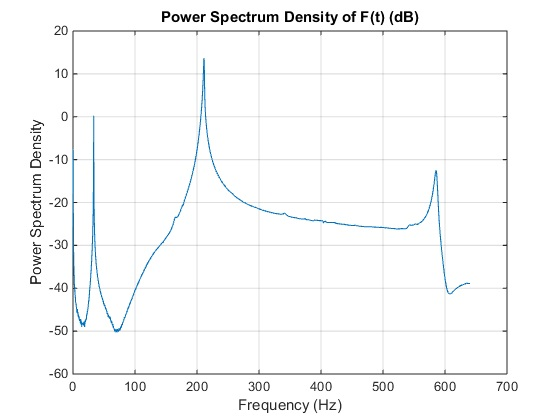
\includegraphics[height=5.50cm]{baseC_wtWeight_ASDoutput.jpg}
		\label{fig:baseC_wtWeight_ASDoutput}
		}
		\quad
		\subfigure[Output ASD for base excitation using corrected data(LOOSE)]
		{
		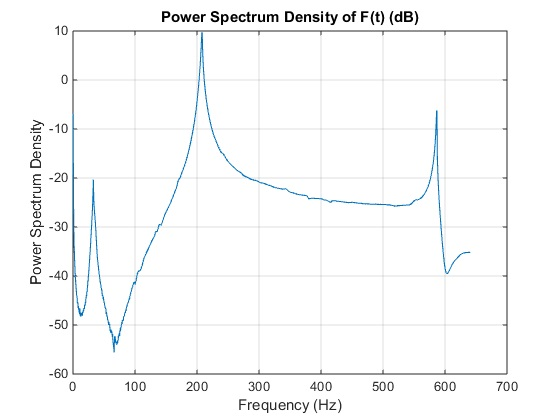
\includegraphics[height=5.50cm]{baseC_woWeight_ASDoutput.jpg}
		\label{fig:baseC_woWeight_ASDoutput}
		}
		\caption{Output ASD plots for base excitation. Results shown for FIXED and LOOSE condition.}
		\label{fig:OutputASDBaseFigs}
	\end{figure}
%
	\begin{figure}[H]
		\centering
		\subfigure[Input ASD for LOC4 excitation using raw data (FIXED)]
		{
		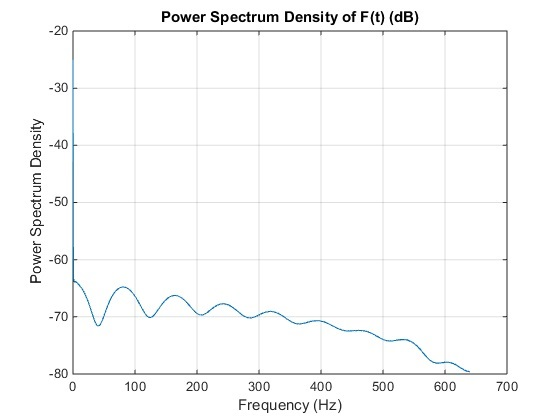
\includegraphics[height=5.50cm]{LOC4R_wtWeight_ASDinput.jpg}
		\label{fig:LOC4R_wtWeight_ASDinput}
		}
		\quad
		\subfigure[Input ASD for LOC4 excitation using raw data (LOOSE)]
		{
		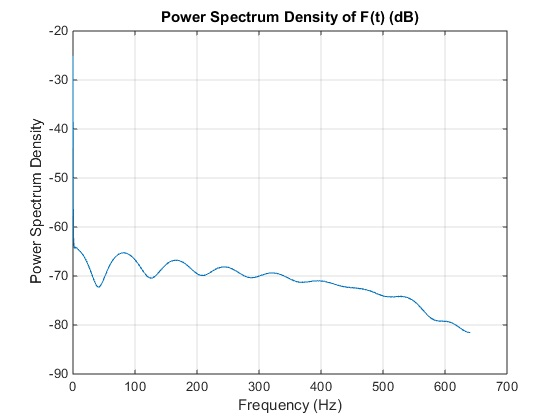
\includegraphics[height=5.50cm]{LOC4R_woWeight_ASDinput.jpg}
		\label{fig:LOC4R_woWeight_ASDinput}
		}
		\quad
		\subfigure[Input ASD for LOC4 excitation using corrected data (FIXED)]
		{
		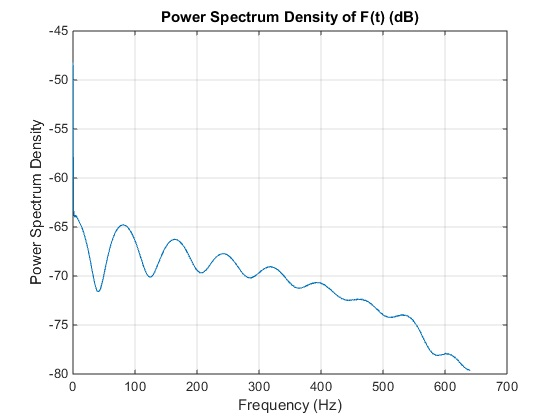
\includegraphics[height=5.50cm]{LOC4C_wtWeight_ASDinput.jpg}
		\label{fig:LOC4C_wtWeight_ASDinput}
		}
		\quad
		\subfigure[Input ASD for LOC4 excitation using corrected data(LOOSE)]
		{
		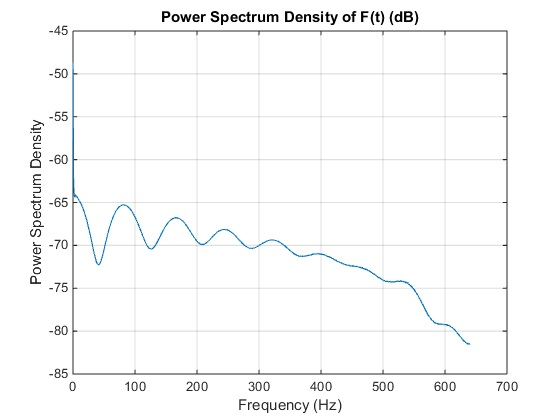
\includegraphics[height=5.50cm]{LOC4C_woWeight_ASDinput.jpg}
		\label{fig:LOC4C_woWeight_ASDinput}
		}
		\caption{Input ASD plots for LOC4 excitation. Results shown for FIXED and LOOSE condition.}
		\label{fig:InputASDLOC4Figs}
	\end{figure}
%
	\begin{figure}[H]
		\centering
		\subfigure[Output ASD for LOC4 excitation using raw data (FIXED)]
		{
		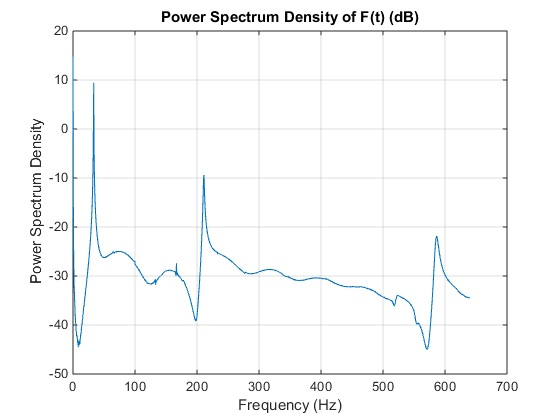
\includegraphics[height=5.50cm]{LOC4R_wtWeight_ASDoutput.jpg}
		\label{fig:LOC4R_wtWeight_ASDoutput}
		}
		\quad
		\subfigure[Output ASD for LOC4 excitation using raw data (LOOSE)]
		{
		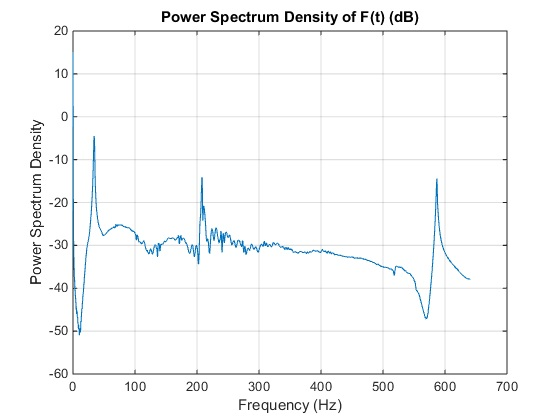
\includegraphics[height=5.50cm]{LOC4R_woWeight_ASDoutput.jpg}
		\label{fig:LOC4R_woWeight_ASDoutput}
		}
		\quad
		\subfigure[Output ASD for LOC4 excitation using corrected data (FIXED)]
		{
		\includegraphics[height=5.50cm]{LOC4C_wtWeight_ASDoutput.jpg}
		\label{fig:LOC4C_wtWeight_ASDoutput}
		}
		\quad
		\subfigure[Output ASD for LOC4 excitation using corrected data(LOOSE)]
		{
		\includegraphics[height=5.50cm]{LOC4C_woWeight_ASDoutput.jpg}
		\label{fig:LOC4C_woWeight_ASDoutput}
		}
		\caption{Output ASD plots for LOC4 excitation. Results shown for FIXED and LOOSE condition.}
		\label{fig:OutputASDLOC4Figs}
	\end{figure}
%
%
\end{document}
